\documentclass[xetex,mathserif,serif,aspectratio=169]{beamer}

\usepackage{xltxtra}
\usepackage{color}
\usepackage{url}
\usepackage{listings}
\usepackage{fontspec}
\usepackage{geometry}
\usepackage{lastpage}
\usepackage{fancyhdr}
\usepackage{amsmath}
\usepackage{amsthm}
\usepackage{amssymb}
\usepackage{blkarray}
\usepackage{multicol}
\usepackage{relsize}
\usepackage{listings}
\usepackage{xunicode}
\usepackage{xltxtra}
\usepackage{color}
\usepackage{url}
\usefonttheme[onlymath]{serif}

\definecolor{solarized@base03}{HTML}{002B36}
\definecolor{solarized@base02}{HTML}{073642}
\definecolor{solarized@base01}{HTML}{586e75}
\definecolor{solarized@base00}{HTML}{657b83}
\definecolor{solarized@base0}{HTML}{839496}
\definecolor{solarized@base1}{HTML}{93a1a1}
\definecolor{solarized@base2}{HTML}{EEE8D5}
\definecolor{solarized@base3}{HTML}{FDF6E3}
\definecolor{solarized@yellow}{HTML}{B58900}
\definecolor{solarized@orange}{HTML}{CB4B16}
\definecolor{solarized@red}{HTML}{DC322F}
\definecolor{solarized@magenta}{HTML}{D33682}
\definecolor{solarized@violet}{HTML}{6C71C4}
\definecolor{solarized@blue}{HTML}{268BD2}
\definecolor{solarized@cyan}{HTML}{2AA198}
\definecolor{solarized@green}{HTML}{859900}
\definecolor{yaleblue}{HTML}{0E4C92}

\newcommand{\yellow}[1]{\textcolor{solarized@yellow}{#1}}
\newcommand{\orange}[1]{\textcolor{solarized@orange}{#1}}
\newcommand{\red}[1]{\textcolor{solarized@red}{#1}}
\newcommand{\magenta}[1]{\textcolor{solarized@magenta}{#1}}
\newcommand{\violet}[1]{\textcolor{solarized@violet}{#1}}
\newcommand{\blue}[1]{\textcolor{solarized@blue}{#1}}
\newcommand{\cyan}[1]{\textcolor{solarized@cyan}{#1}}
\newcommand{\green}[1]{\textcolor{solarized@green}{#1}}
\newcommand{\yblue}[1]{\textcolor{yaleblue}{#1}}
\newcommand{\base}[1]{\textcolor{solarized@base01}{#1}}


\defaultfontfeatures{Mapping=tex-text}
\hypersetup{pdfstartview={FitH}}

\newcommand{\old}[1]{\fontspec[Alternate=1,Ligatures={Common}]{Hoefler Text}\fontsize{18pt}{30pt}\selectfont #1}%
\newcommand{\oldA}[1]{\fontspec[Alternate=1,Ligatures={Common, Rare}]{Hoefler Text}\fontsize{12pt}{15pt}\selectfont #1}%
\newcommand{\oldB}[1]{\fontspec[Ligatures={Common}]{Didot}\fontsize{12pt}{15pt}\color{solarized@base02}\selectfont #1}%
\newcommand{\tfont}[1]{\fontspec[Alternate=1,Ligatures={Common}]{Hoefler Text}\fontsize{12pt}{20pt}\selectfont #1}%
\newcommand{\dfont}[1]{\fontspec[Ligatures={Common}]{Didot}\fontsize{12pt}{12pt}\selectfont #1}%

\setbeamerfont{title}{family=\old}
\setbeamerfont{author}{family=\tfont}%
\setbeamerfont{frametitle}{family=\oldA}
\setbeamerfont{date}{family=\dfont}

\setbeamertemplate{navigation symbols}{}
\setbeamertemplate{footline}[text line]{%
  \parbox{0.99\linewidth}{
    \normalsize\vspace*{-24pt}\hfill{\color{solarized@base00}\insertframenumber/\inserttotalframenumber}
  }
}


\setlength{\parindent}{0pt}
\setlength{\parskip}{12pt}

\setbeamercolor{structure}{bg=solarized@base3, fg=solarized@base02}
\setbeamercolor{titlelike}{fg=solarized@cyan}
\setbeamercolor{title}{fg=solarized@blue}
\setbeamercolor{subtitle}{fg=solarized@magenta}
\setbeamercolor{alerted text}{fg=orange}
\setbeamercolor{itemize}{fg=solarized@base02}
\setbeamercolor{background canvas}{bg=solarized@base3}
\setbeamercolor{enumerate subitem}{fg=solarized@base02}

\newcommand{\minimize}{\mathop{\mathrm{minimize}}}
\newcommand{\argmin}{\mathop{\mathrm{arg\,min}}}
\newcommand{\argmax}{\mathop{\mathrm{arg\,max}}}
\newcommand{\st}{\mathop{\mathrm{subject\,\,to}}}


\usepackage[]{algorithm2e}
\usepackage{../kbordermatrix}

\begin{document}

%%%%%%%%%%%%%%%%%%%%%%%%%%%%%%%%%%%%%%%%%%%%%%%%%%%
\begin{frame}[fragile] \frametitle{} \oldB \small

\vfill

{\fontsize{0.7cm}{0cm}\selectfont Lecture 17 \\\vspace{0.2cm}
Convolutional Neural Networks}\\\vspace{0.5cm}
30 March 2016

\vspace{2cm}

\begin{minipage}{0.6\textwidth}
Taylor B. Arnold \\
Yale Statistics \\
STAT 365/665
\end{minipage}
\hfill
\begin{minipage}{0.3\textwidth}\raggedleft

\includegraphics[scale=0.3]{../yale-logo.png}
\end{minipage}%

\end{frame}

%%%%%%%%%%%%%%%%%%%%%%%%%%%%%%%%%%%%%%%%%%%%%%%%%%%
\begin{frame}[fragile] \frametitle{} \oldB \small

Notes:
\begin{itemize}
\item Problem set 6 is online and due \textbf{next} Friday, April 8th
\item Problem sets 7,8, and 9 will be due on the remaining Fridays
\item No class on April 11th or 13th
\end{itemize}

\end{frame}

%%%%%%%%%%%%%%%%%%%%%%%%%%%%%%%%%%%%%%%%%%%%%%%%%%%
\begin{frame}[fragile] \frametitle{} \oldB \small

\textbf{\yblue{Convolutional Neural Networks}}

Convolution layers are a slightly more exotic variant on the dense
linear layers we have been using so far. They simultaneously address
several issues that are commonly seen in computer vision applications: \pause
\begin{itemize}
\item We want to utilize the known geometry of the data (color channels
and locality) \pause
\item Larger images require an enormous number of weights for even modestly
sized hidden layers. Using 96x96 pixel images and a single hidden layer with
$1024$ nodes, requires just under ten million individual weights! \pause
\item Many applications require detecting or recognizing items that may be
placed differently in the image field; it will be useful to have a method
that is insensitive to small shifts in the individual pixels.
\end{itemize}
I'll restrict today's discussion to 2D-convolutions, as they are generally
used in image processing, but note that they can also be applied to 1D, 3D
and higher dimensions (we'll use 1D in the text analysis applications).

\end{frame}

%%%%%%%%%%%%%%%%%%%%%%%%%%%%%%%%%%%%%%%%%%%%%%%%%%%
\begin{frame}[fragile] \frametitle{} \oldB \small

\textbf{\yblue{Convolutional Neural Networks, cont.}}

We can think of convolutional layers as being the same as a dense/linear
layer, with two constraints applied to the weights and biases.
\begin{itemize}
\item Sparsity with local receptive field: the weight and biases for a given neuron
are only non-zero over a small, local region of the input image.
\item Shared weights: the non-zero weights and biases are the same across all of the
neurons, up to a shifting over the image.
\end{itemize}
A picture should make this much more clear.

\end{frame}

%%%%%%%%%%%%%%%%%%%%%%%%%%%%%%%%%%%%%%%%%%%%%%%%%%%
\begin{frame}[fragile] \frametitle{} \oldB \small

\begin{center}
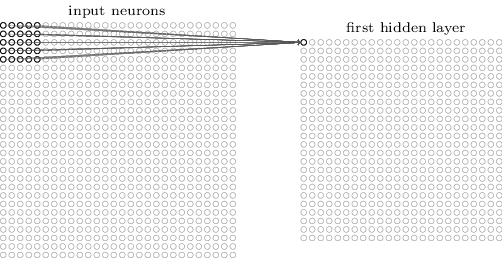
\includegraphics[height=0.7\textheight]{img/tikz44.png}
\end{center}

\end{frame}

%%%%%%%%%%%%%%%%%%%%%%%%%%%%%%%%%%%%%%%%%%%%%%%%%%%
\begin{frame}[fragile] \frametitle{} \oldB \small

\begin{center}
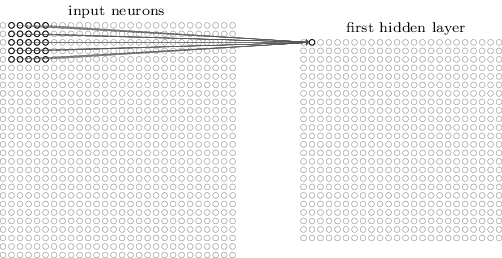
\includegraphics[height=0.7\textheight]{img/tikz45.png}
\end{center}

\end{frame}

%%%%%%%%%%%%%%%%%%%%%%%%%%%%%%%%%%%%%%%%%%%%%%%%%%%
\begin{frame}[fragile] \frametitle{} \oldB \small

\textbf{\yblue{Filters}}

What we have just described is what we call a filter; a
convolutional layer is made up of some predetermined
number of filters. That is, we have multiple set of local
weights that are applied over small chunks of the image.
These allow us to capture different components that may
all be useful for the classification task at hand.

\end{frame}

%%%%%%%%%%%%%%%%%%%%%%%%%%%%%%%%%%%%%%%%%%%%%%%%%%%
\begin{frame}[fragile] \frametitle{} \oldB \small

\textbf{\yblue{Filters: History}}

The idea of using a filter on images is not a new idea to
neural networks; the difference here is the filters are
adaptively learned from data.

For example, take the following fixed kernel weights:
\begin{align*}
\left(\begin{array}{cc} 1 & 0 \\ 0 & -1 \end{array} \right)
\end{align*}
What happens when we apply this over an image?

\end{frame}

%%%%%%%%%%%%%%%%%%%%%%%%%%%%%%%%%%%%%%%%%%%%%%%%%%%
\begin{frame}[fragile] \frametitle{} \oldB \small

\begin{center}
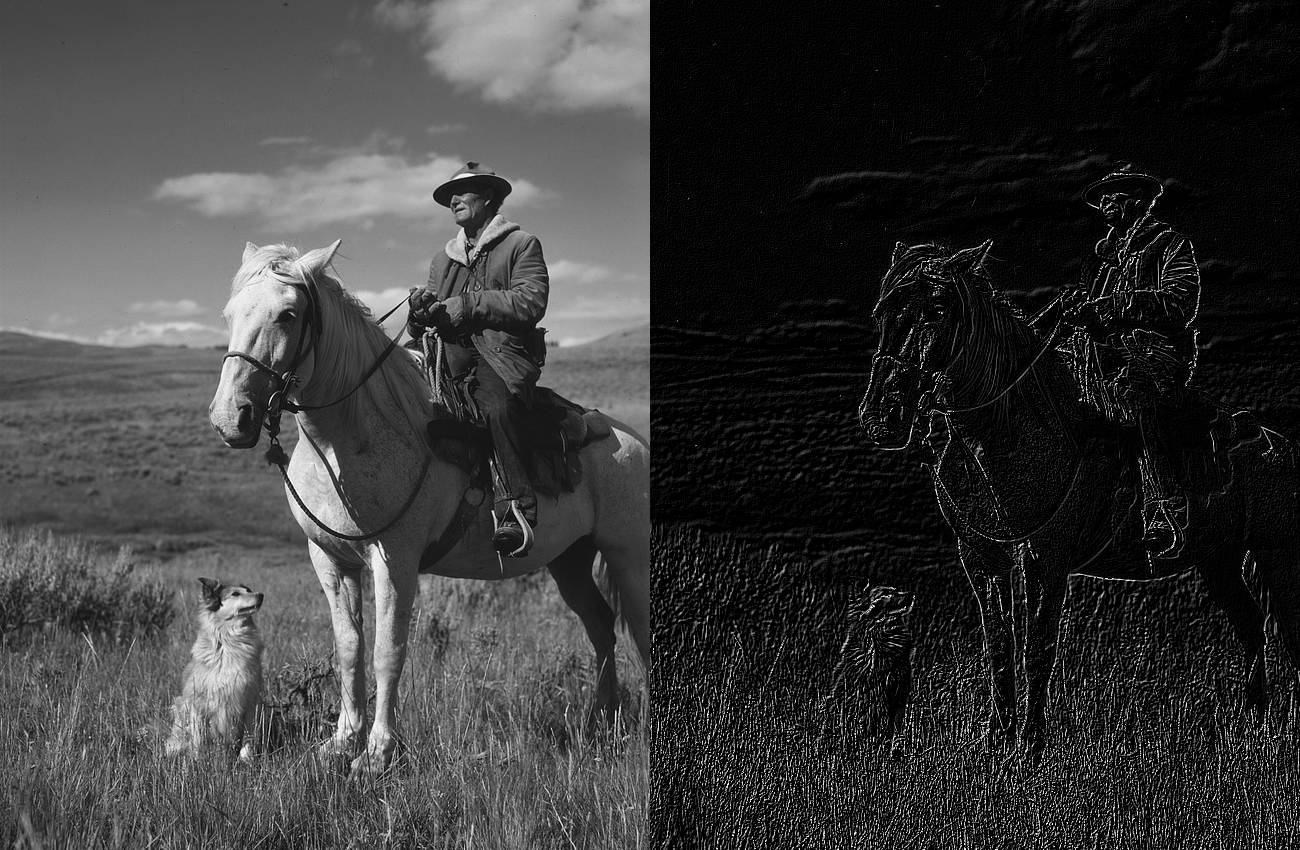
\includegraphics[height=0.7\textheight]{img/both.jpg}
\end{center}

\end{frame}

%%%%%%%%%%%%%%%%%%%%%%%%%%%%%%%%%%%%%%%%%%%%%%%%%%%
\begin{frame}[fragile] \frametitle{} \oldB \small

\begin{center}
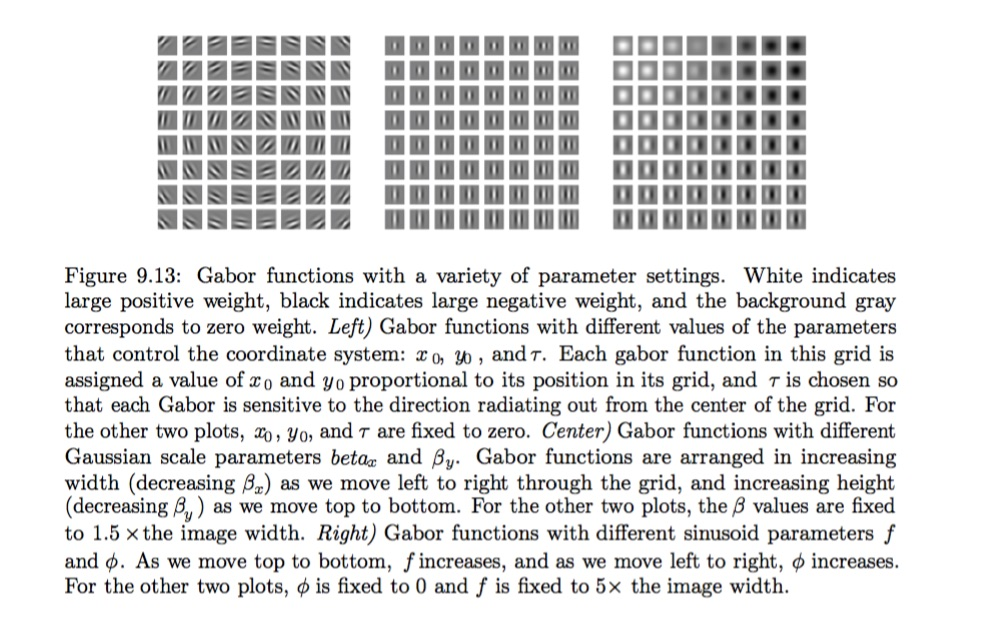
\includegraphics[height=0.8\textheight]{img/gabor.jpg}
\end{center}

\end{frame}

%%%%%%%%%%%%%%%%%%%%%%%%%%%%%%%%%%%%%%%%%%%%%%%%%%%
\begin{frame}[fragile] \frametitle{} \oldB \small

A convolutional layer with $3$ filters:

\begin{center}
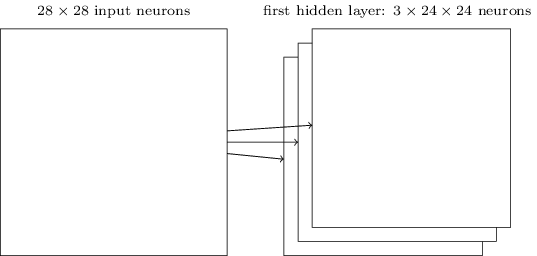
\includegraphics[height=0.7\textheight]{img/tikz46.png}
\end{center}

\end{frame}

%%%%%%%%%%%%%%%%%%%%%%%%%%%%%%%%%%%%%%%%%%%%%%%%%%%
\begin{frame}[fragile] \frametitle{} \oldB \small

\textbf{\yblue{Zero padding}}

You may have noticed that the grid of pixels of the output image
will have fewer rows and columns than the input image.
In some cases this is okay, but it is often advantageous to
preserve the size of the grid (there are several reasons that we
want to grid size to be divisible by $2^n$ for some reasonably large
$n$). To do so, we can add extra rows and columns of zeros
(zero padding) to the input before applying the

\end{frame}

%%%%%%%%%%%%%%%%%%%%%%%%%%%%%%%%%%%%%%%%%%%%%%%%%%%
\begin{frame}[fragile] \frametitle{} \oldB \small

\textbf{\yblue{Kernel and stride}}

The architecture of a (2D) convolution layer is primarily
determined by four numbers:
\begin{enumerate}
\item the number of filters, F
\item the height of the kernel, $k_h$
\item the width of the kernel, $k_w$
\item the stride, $k_s$
\end{enumerate}
The stride tells us how far the local set of weights is
shifted before being applied. We'll mostly use a stride
of $1$, but just note that other values are possible.

\end{frame}

%%%%%%%%%%%%%%%%%%%%%%%%%%%%%%%%%%%%%%%%%%%%%%%%%%%
\begin{frame}[fragile] \frametitle{} \oldB \small

A 5x5 kernel:

\begin{center}
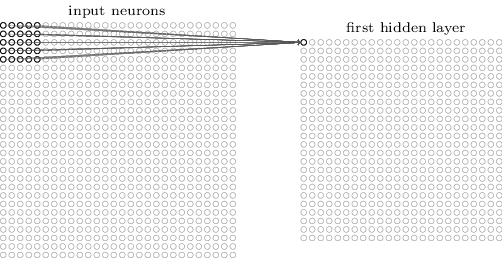
\includegraphics[height=0.7\textheight]{img/tikz44.png}
\end{center}

\end{frame}

%%%%%%%%%%%%%%%%%%%%%%%%%%%%%%%%%%%%%%%%%%%%%%%%%%%
\begin{frame}[fragile] \frametitle{} \oldB \small

A stride of $1$:

\begin{center}
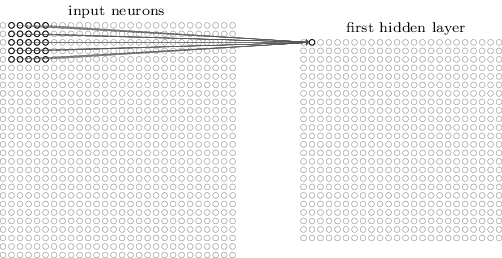
\includegraphics[height=0.7\textheight]{img/tikz45.png}
\end{center}

\end{frame}

%%%%%%%%%%%%%%%%%%%%%%%%%%%%%%%%%%%%%%%%%%%%%%%%%%%
\begin{frame}[fragile] \frametitle{} \oldB \small

A nice demo of applying convolution over a grid using alternative
strides and zero padding:

\begin{center}
\url{http://cs231n.github.io/assets/conv-demo/index.html}
\end{center}

\end{frame}

%%%%%%%%%%%%%%%%%%%%%%%%%%%%%%%%%%%%%%%%%%%%%%%%%%%
\begin{frame}[fragile] \frametitle{} \oldB \small

\textbf{\yblue{Tensors}}

A convolution can also be described in purely algebraic
terms. We are defining a map from a three dimensional space
to a three dimensional space:
\begin{align*}
F^1 \times W^1 \times H^1 \rightarrow F^2 \times W^2 \times H^2
\end{align*}
Where $F$ is the number of filters, $W$ the width of the image,
and $H$ the height of the image. You can now see why tensors are
considered a generalization of a matrix operations, and why they
are so important in learning neural network models.

\pause The value $F^1$ is equal to one for the MNIST dataset, but
for CIFAR-10 we would set it to $3$ to deal with the $3$ color
channels.

\end{frame}

%%%%%%%%%%%%%%%%%%%%%%%%%%%%%%%%%%%%%%%%%%%%%%%%%%%
\begin{frame}[fragile] \frametitle{} \oldB \small

\textbf{\yblue{Pooling layers}}

Convolutional neural networks have another type of layer that can
also be described by applying a function locally to small section
of the image. These layers are called pooling layers; they differ
from convolution layers because:
\begin{itemize}
\item they have no learned weights
\item may not be linear functions of their inputs
\item are applied separately to each kernel
\item the stride is usually equal to the size of the kernel; that is,
the regions are non-overlapping
\end{itemize}
The most common type of pooling (by far) is called max-pooling, with
a 2x2 kernel and stride of $2$.
This halves the extent of each dimension (reduces the
number of data points by a factor of $4$ for 2D images) and can greatly
decrease the learning time and improve over-fitting of the data.

\end{frame}

%%%%%%%%%%%%%%%%%%%%%%%%%%%%%%%%%%%%%%%%%%%%%%%%%%%
\begin{frame}[fragile] \frametitle{} \oldB \small

Max pooling using a 2x2 filter and a stride of $2$:

\begin{center}
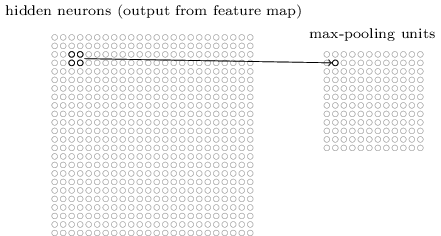
\includegraphics[height=0.7\textheight]{img/tikz47.png}
\end{center}

\end{frame}

%%%%%%%%%%%%%%%%%%%%%%%%%%%%%%%%%%%%%%%%%%%%%%%%%%%
\begin{frame}[fragile] \frametitle{} \oldB \small

An example of convolution followed by max pooling:

\begin{center}
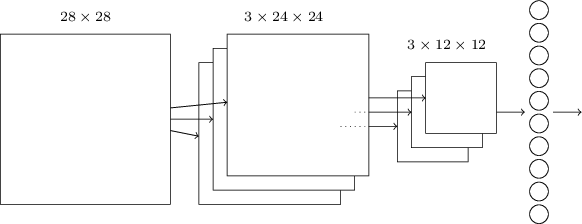
\includegraphics[height=0.5\textheight]{img/tikz49.png}
\end{center}

\end{frame}

%%%%%%%%%%%%%%%%%%%%%%%%%%%%%%%%%%%%%%%%%%%%%%%%%%%
\begin{frame}[fragile] \frametitle{} \oldB \small

Let's now apply convolutional networks to the MNIST dataset using
the keras library.

\end{frame}

%%%%%%%%%%%%%%%%%%%%%%%%%%%%%%%%%%%%%%%%%%%%%%%%%%%
\begin{frame}[fragile] \frametitle{} \oldB \small

A demo of applying convolutional neural networks to the MNIST dataset:

\begin{center}
\url{http://cs.stanford.edu/people/karpathy/convnetjs/demo/mnist.html}
\end{center}

\end{frame}





\end{document}







